\documentclass[../../main.tex]{subfiles}
% \graphicspath{{\subfix{../images/}}}

\begin{document}
\subsection{¿Qué es una Evaluación de Impacto?}
\begin{comment}
El uso de métodos cuantitativos para medir el impacto de programas sociales ha cobrado un gran interés en los últimos años \cite{bernal}. Las evaluaciones de impacto han comenzado a desempeñar un papel preponderante en el diseño de políticas públicas \cite{bernal}.
\end{comment}

Los programas y políticas de desarrollo suelen estar diseñados para cambiar resultados, como aumentar los ingresos, mejorar el aprendizaje o reducir las enfermedades \cite{gertler-2016}. Saber si estos cambios se logran o no es una pregunta crucial para las políticas públicas \cite{gertler-2016}, y aquí es donde entra en juego lo que se conoce como \textbf{evaluación de impacto}.

Una evaluación de impacto mide los cambios en el bienestar de los individuos que se pueden atribuir a un proyecto, un programa o una política específicos \cite{gertler-2016}. Su sello distintivo radica en que pueden proporcionar \textbf{evidencia} robusta y creíble sobre si un programa concreto ha alcanzado o está alcanzando sus resultados deseados \cite{gertler-2016}. 

Este tipo de evaluaciones pone un fuerte énfasis en los resultados y busca responder una pregunta específica de causa y efecto: ¿cuál es el impacto (o efecto causal) de un programa en un resultado de interés? \cite{gertler-2016}. Es decir, se focalizan en los cambios directamente atribuibles al tratamiento \cite{gertler-2016} sobre un conjunto de \textbf{variables de resultado} o \textbf{de interés} en un conjunto de individuos \cite{bernal}. Estas variables son aquellas sobre las cuales se espera que el programa tenga un efecto en los beneficiarios \cite{bernal}. Por ejemplo, podrían ser la estatura y peso de los individuos, o la cantidad de empleados o de ventas en una empresa.

Por lo tanto, el objetivo final de la evaluación de impacto consiste en establecer la diferencia entre la variable de resultado del individuo participante en el programa en presencia del programa, y la variable de resultado de ese individuo en ausencia del programa \cite{bernal}, lo que se conoce como \textbf{efecto del tratamiento}. Sin embargo, es evidente que la respuesta a ``¿qué habría pasado con los beneficiarios en ausencia del programa?'' se refiere a una situación que no es observable. Este resultado hipotético se denomina \textbf{contrafactual} y es lo que se debe estimar en cualquier evaluación de impacto.

Algunas de las principales razones por las que se debería promover el uso de estas evaluaciones como herramientas de gestión provienen del hecho que permiten mejorar la rendición de cuentas, la inversión de recursos públicos o la efectividad de una política, obtener financiamiento, como así también probar modalidades de programas alternativos o innovaciones de diseño \cite{gertler-2016} y revelar la realidad de muchas políticas públicas para de esta forma contribuir a la fiscalización mediática \cite{bernal}.

Un ejemplo claro de por qué son necesarias las evaluaciones de impacto es el que describe Howard White con respecto al Programa Integrado de Nutrición en Bangladesh (PINB) \cite{white2009theory}. Este programa identificaba, mediante mediciones en campo, a los niños desnutridos y los asignaba a un tratamiento que incluía alimentación suplementaria a los menores y educación nutricional a las madres \cite{bernal}. Inicialmente, el programa fue considerado como un éxito ya que los datos de monitoreo mostraban caídas importantes en los niveles de desnutrición. El Banco Mundial decidió, con base en esta evidencia y previo a cualquier tipo de evaluación, aumentar los recursos destinados al programa. Sin embargo, las primeras evaluaciones de impacto, realizadas por el Grupo Independiente de Evaluación del mismo Banco Mundial y por la ONG inglesa \textit{Save the Children}, mostraron que la mejoría de los indicadores de los beneficiarios era similar o inferior a la de otros niños con características comparables que no hacían parte del programa \cite{bernal}. Estos resultados reflejaron que las percepciones de los administradores del programa y de las entidades financiadoras eran erradas, y sugirieron algunos correctivos al programa \cite{bernal}.

\begin{comment}
    AGREGAR EL EJEMPLO DE MEXICO QUE APARECE EN EL GERTLER
\end{comment}

% Preparación de una evaluación?

\subsection{Estimación del Tratamiento}
El marco teórico estándar para formalizar el problema de la evaluación de impacto se basa en el modelo de resultado \textit{potencial} o modelo de Roy-Rubin \cite{rubin1974}. 

Formalmente, definimos dos elementos para cada individuo \(i = 1,...,N\), donde \(N\) denota la población total:
\begin{itemize}
    \item Por un lado, el indicador de tratamiento \(D_i\), tal que \(D_i = 1\) implica que el individuo \(i\) participó del tratamiento, y \(D_i = 0\) en caso contrario.
    \item Por otro lado, las variables de resultado las definimos como \(Y_i(D_i) = Y_i|D_i\) - se lee como ``el valor de \(Y_i\) \textit{dado} \(D_i\)''. De esta forma, \(Y_i(1)\) es la variable de resultado si el individuo \(i\) es tratado, e \(Y_i(0)\) es la variable de resultado si el individuo \(i\) no es tratado.
\end{itemize}

Con esto, el \textbf{efecto del tratamiento} para un individuo \(i\) se puede escribir como:
\begin{equation}
    \tau_i = Y_i(1) - Y_i(0) = (Y_i|D_i=1) - (Y_i|D_i=0)
    \label{eq:ite} % ite = individual treatment effect
\end{equation}

Según esta fórmula, el impacto causal (\(\tau\)) de un programa (\(D\)) en una variable resultado (\(Y\)) para un individuo \(i\) es la diferencia entre la variable con el programa (\(Y_i(1)\)) y la misma variable sin el programa (\(Y_i(0)\)). 

De nuevo, el problema fundamental de la evaluación de impacto es que se intenta medir una variable en un mismo momento del tiempo para la misma unidad de observación pero en dos realidad diferentes \cite{gertler-2016}. Sin embargo, claramente solo se da uno de los dos resultados potenciales \(Y_i(1)\) o \(Y_i(0)\), pero no ambos. Es decir, en los datos queda solamente registrado \(Y_i(1)\) si \(D_i=1\) y \(Y_i(0)\) si \(D_i=0\); no se dispone de \(Y_i(1)\) si el individuo no fue tratado (\(D_i=0\)), ni tampoco de \(Y_i(0)\) si el individuo fue tratado (\(D_i=1\)). De esta manera, el \textbf{resultado observado} de \(Y_i\) se puede expresar como:

\begin{equation}
    Y_i = D_i Y_i(1) + (1-D_i)Y_i(0) =
    \begin{cases}
        Y_i(1) \text{ si } D_i=1 \\
        Y_i(0) \text{ si } D_i=0
    \end{cases}
    \label{eq:observed-result}
\end{equation}

En la ecuación \ref{eq:ite}, el término \(Y_i(0) = Y_i|D_i=0\) representa el contrafactual, es decir \textit{cuál habría sido el resultado si la unidad no hubiera participado en el programa}. Al ser imposible observar directamente el contrafactual, es necesario \textbf{estimarlo}. La forma más directa de solucionar este problema sería hallando un ``clon perfecto'' para cada uno de los individuos participantes del programa, lo cual resulta bastante difícil. Por lo tanto, el primer paso para lograr esta estimación consiste en \textbf{desplazarse desde el nivel individual al nivel del grupo} \cite{gertler-2016}, concentrando el análisis en el impacto o efecto \textit{promedio} (y no individual).

En primera instancia, se puede estimar el \textit{impacto promedio del programa \textbf{sobre la población}} (o \(ATE\)):

\begin{equation}
    ATE = \mathbb{E}\left[Y_i(1)-Y_i(0)\right]
\end{equation}

El \(ATE\) se interpreta como el cambio promedio en la variable de resultado cuando un individuo escogido al azar pasa aleatoriamente de ser participante a ser no participante \cite{bernal}. Esta medida es relevante en el caso de la evaluación de un programa universal. Sin embargo, en la mayoría de los casos, el tratamiento solo está disponible para un subconjunto de la población. En este caso, es posible utilizar un estimador que únicamente promedie el efecto sobre la población elegible \cite{bernal}. 

De esta forma, definimos el \textit{impacto promedio del programa \textbf{sobre los tratados}} (o \(ATT\)), que es en general el parámetro de mayor interés en una evaluación de impacto, y representa el efecto esperado del tratamiento en el subconjunto de individuos que fueron efectivamente tratados:

\begin{equation}
    ATT = \mathbb{E} \left[Y_i(1)-Y_i(0)|D_i=1\right] = \mathbb{E} \left[Y_i(1)|D_i=1\right] - \mathbb{E} \left[Y_i(0)|D_i=1\right]
    \label{eq:ATT}
\end{equation}

Es decir, el \(ATT\) es la diferencia entre la media de la variable de resultado en el grupo de los participantes y la media que hubieran obtenido los participantes si el programa no hubiera existido \cite{bernal}.

Notemos que podemos reescribir la ecuación \ref{eq:ATT} de la siguiente manera:
\begin{equation}
    ATT + \mathbb{E} \left[Y_i(0)|D_i=1\right] = \mathbb{E} \left[Y_i(1)|D_i=1\right] 
    \label{eq:ATT2}
\end{equation}

Si ahora restamos \(\mathbb{E} \left[Y_i(0)|D_i=0\right]\) a ambos lados, obtenemos:
\begin{equation}
    ATT + \mathbb{E} \left[Y_i(0)|D_i=1\right] - \mathbb{E} \left[Y_i(0)|D_i=0\right]\ = \mathbb{E} \left[Y_i(1)|D_i=1\right] - \mathbb{E} \left[Y_i(0)|D_i=0\right]\
    \label{eq:ATT3}
\end{equation}

De aquí se deduce que utilizar \(\mathbb{E} \left[Y_i(0)|D_i=0\right]\) como aproximación del contrafactual \(\mathbb{E} \left[Y_i(0)|D_i=1\right]\) permite recuperar el \(ATT\) si y solo si:
\begin{equation}
    \mathbb{E} \left[Y_i(0)|D_i=1\right]\ - \mathbb{E} \left[Y_i(0)|D_i=0\right]\ = 0
    \label{eq:supuesto1}
\end{equation}

Dicho esto, el principal reto de la evaluación de impacto es justamente determinar las condiciones bajo las cuales se cumple \ref{eq:supuesto1}, es decir que \(\mathbb{E} \left[Y_i(0)|D_i=0\right]\) sea una aproximación válida de \(\mathbb{E} \left[Y_i(0)|D_i=1\right]\) \cite{bernal}.

\subsection{El Grupo de Control como Estimador del Contrafactual}
En la ecuación \ref{eq:ATT}, el término \(\mathbb{E} \left[Y_i(1)|D_i=1\right]\) es un resultado observable mientras que \(\mathbb{E} \left[Y_i(0)|D_i=1\right]\) es el promedio contrafactual que debemos aproximar. Para ello, se construye lo que se conoce como grupo de control, formado por individuos que no participan del programa pero que, idealmente, son estadísticamente similares \cite{gertler-2016} al grupo de tratamiento, compuesto por quienes sí recibieron el programa.

\begin{figure}[h!]
    \centering
    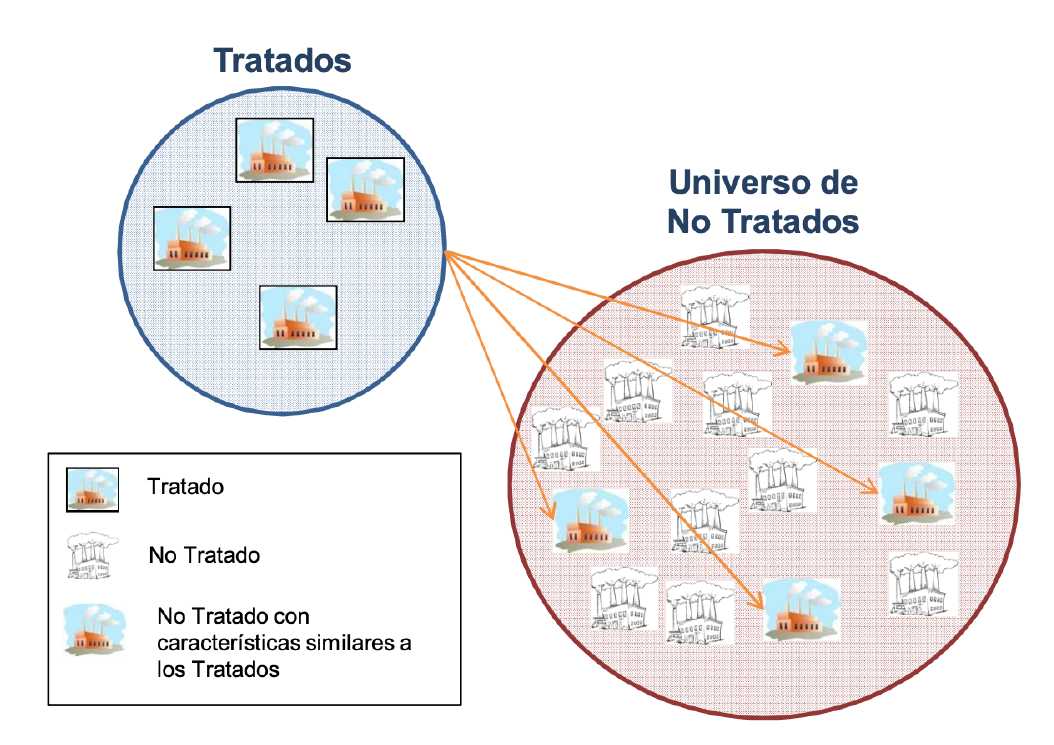
\includegraphics[width=0.6\textwidth]{figs/grupo-de-control.png}
    \caption{}
    \label{fig:control-group}
\end{figure}

Por lo tanto, en la práctica, el reto de una evaluación de impacto es definir un \textit{buen} grupo de control, es decir uno que sea estadísticamente idéntico al de tratamiento, en promedio, en ausencia del programa \cite{gertler-2016}. Si se lograra que los dos grupos sean idénticos, con la única excepción que un grupo participa del programa y el otro no, entonces sería posible estar seguros que cualquier diferencia en los resultados tiene que deberse al programa \cite{gertler-2016}.

Para que un grupo de comparación sea válido, debe satisfacer lo siguiente \cite{gertler-2016}:
\begin{itemize}
    \item Las características \textit{promedio} del grupo de tratamiento y del grupo de comparación deben ser idénticas en ausencia del programa. Cabe resaltar que no es necesario que las unidades individuales en el grupo de tratamiento tengan clones perfectos en el grupo de control.
    \item No debe ser afectado por el tratamiento de forma directa ni indirecta.
    \item El grupo de comparación debería reaccionar de la misma manera que el grupo de tratamiento si fuera objeto del programa.
\end{itemize}

Cuando el grupo de comparación no produce una estimación precisa del contrafactual, no se puede establecer el verdadero impacto del programa. A continuación, se presentan dos situaciones en las que el grupo de comparación seleccionado conduce a una estimación incorrecta del contrafactual.

\subsubsection{Comparaciones antes-después}
Este tipo de comparaciones intenta establecer el impacto de un programa a partir de un seguimientos de los cambios en los resultados en los participantes del programa a lo largo del tiempo. Consideran el contrafactual como el resultado para el grupo de tratamiento antes que comience la intervención, momento también conocido como \textbf{línea de base}. Esta comparación supone que si el programa no hubiera existido, el resultado para los participantes del programa habría sido igual a su situación antes del programa, lo cual en la mayoría de los tratamientos este supuesto no puede sostenerse \cite{gertler-2016}.

\subsubsection{Comparaciones de inscritos y no inscritos: Sesgo de autoselección}
Una de las formas más directas de solucionar el problema del contrafactual podría ser simplemente utilizar el promedio de la variable de resultado entre los individuos no participantes del programa pero elegibles para participar. Es decir, se estaría usando a \(\mathbb{E} \left[Y_i(0)|D_i=0\right]\), que sí se puede observar, como una aproximación de \(\mathbb{E} \left[Y_i(0)|D_i=1\right]\) \cite{bernal}. Sin embargo, esto podría generar estimaciones inexactas del efecto del programa, dado que los participantes y los no participantes generalmente son diferentes (en características observadas y no observadas), aún en ausencia del programa, y es justamente por tal motivo que unos \textit{eligen} participar y otros no \cite{bernal}. Este problema se conoce como \textbf{sesgo de autoselección}, ya que el grupo se \textit{autoselecciona} para no participar de un programa. Más concretamente, este sesgo se produce cuando los motivos por los que un individuo participa en un programa, usualmente no observables y difíciles de medir, están correlacionados con los resultados \cite{gertler-2016}, y por ende, es muy probable que la variable de resultado del grupo de tratamiento y del grupo de control sean diferentes, \textit{aún si el programa no existiera} \cite{bernal}.

A modo de ejemplo, se puede pensar en un programa de nutrición infantil. Podría ocurrir que las madres de familia participantes del programa sean más proactivas respecto al desarrollo de sus hijos, por lo cual se preocuparon en lograr la participación en el programa. El problema de autoselección en este caso radica en que la motivación de las madres (que no se observa y es difícil de medir) afecta no solo la probabilidad de participar en el programa, sino también el estado nutricional de los niños ya que estas podrían vigilar mejor la dieta de sus hijos. De esta forma, la diferencia observada en el estado nutricional de los niños de los dos grupos podría deberse parcialmente a la diferencia en el nivel de compromiso de las madres, y no exclusivamente a que un grupo participa en el programa y el otro no \cite{bernal}.

\begin{comment}
Es importante en este punto identificar claramente los diferentes resultados que hemos mencionado hasta el momento, los cuales se encuentran en la tabla \ref{tab:different-estimations}.

\begin{table}[h]
    \centering
    \begin{tabular}{p{7cm}m{7cm}}  % Set fixed column widths
        \hline
        \textbf{Lo que se desea medir} (efecto promedio sobre los tratados, \(ATT\)) & \(\mathbb{E} \left[Y_i(1)-Y_i(0)|D_i=1\right]\) \\
        \hline
        \textbf{Lo que observamos} (el promedio de la diferencia entre los resultados de los tratados y el grupo de control) & \(\mathbb{E} \left[Y_i(1)-C_i(0)\right]\) \\
        \hline
        \textbf{El promedio de la diferencia potencial entre lo que observamos y lo que se desea medir} (``sesgo de selección'') & \(\mathbb{E} \left[\left(Y_i(1)-Y_i(0)\right) - \left(Y_i(1)-C_i(0)\right)\right] = \mathbb{E} \left[C_i(0)-Y_i(0)\right]\) \\
        \hline
    \end{tabular}
    \caption{Your caption here}
    \label{tab:different-estimations}
\end{table}
\end{comment}


% Los distintos tipos de experimentos?
\bigskip
Las reglas de un programa para seleccionar a los participantes, también llamadas \textbf{reglas de asignación}, constituyen el parámetro clave para determinar el método de evaluación de impacto. A continuación, presentamos las distintas reglas y los métodos de evaluación que se utilizan en la práctica la trabajar con cada una de ellas.

\subsection{Evaluaciones Experimentales o Aleatorias}
En este tipo de evaluaciones, los beneficiarios del programa en cuestión son seleccionados al azar, es decir mediante un sorteo. De esta forma, todas las unidades elegibles tienen la misma probabilidad de ser seleccionadas para el programa.

La asignación aleatoria se considera la regla de oro de la evaluación de impacto ya que no solo proporciona a los administradores del programa una regla imparcial y transparente para asignar recursos escasos entre poblaciones igualmente merecedoras de ellos, sino que también representa el método más sólido para evaluar el impacto de un programa \cite{gertler-2016}. 

Como explicamos anteriormente, el grupo de comparación ideal sería lo más similar posible al grupo de tratamiento en todos los sentidos, excepto con respecto a su participación en el programa que se evalúa. Ahora bien, el proceso de asignación aleatoria producirá dos grupos que tienen una alta probabilidad de ser estadísticamente idénticos en todas sus características (observables y no observables), siempre que el número de unidades sea suficientemente grande \cite{gertler-2016}. Esto es así ya que en general, si la población de unidades elegibles es lo suficientemente grande, este mecanismo asegura que cualquier rasgo de la población se transfiera a ambos grupos. Dicho esto, lo que ocurre en estos casos es que todos aquellos individuos que no resultaron ser beneficiarios del programa conforman un grupo de control que resulta ser naturalmente un excelente estimador del contrafactual \(\mathbb{E} \left[Y_i(0)|D_i=1\right]\). Es decir, mediante este tipo de asignación, se asegura que:

\begin{equation}
    \mathbb{E} \left[Y_i(0)|D_i=1\right]\ = \mathbb{E} \left[Y_i(0)|D_i=0\right]\
    \label{eq:asig_aleatoria}
\end{equation}

La asignación aleatoria puede utilizarse como regla de asignación de un programa en dos escenarios específicos: cuando la población elegible es mayor que el número de plazas disponibles del programa, o  cuando sea necesario ampliar un programa de manera progresiva hasta que cubra a toda la población elegible \cite{gertler-2016}. Además, la asignación aleatoria podría hacerse a nivel individual (por ejemplo, a nivel de hogares), o a nivel de conglomerado (por ejemplo, comunidades) \cite{bernal}.

Una vez que se haya asignado el tratamiento de manera aleatoria, gracias a \ref{eq:asig_aleatoria}, es bastante sencillo estimar el impacto del programa. Después de que el programa ha funcionado durante un tiempo, tendrán que medirse los resultados de las unidades de tratamiento y de comparación. El impacto del programa es sencillamente la diferencia entre el resultado promedio para el grupo de tratamiento y el resultado promedio para el grupo de comparación, es decir:

\[
\mathbb{E} \left[Y_i(1)|D_i=1\right]\ - \mathbb{E} \left[Y_i(0)|D_i=0\right]\
\]


\subsection{Evaluaciones Cuasiexperimentales}
\begin{comment}
    Profundizar en diferencias en diferencias y en PSM
    Mencionar variables instrumentales y regresión discontinua
\end{comment}

\subsubsection{Diferencias en Diferencias}

\subsubsection{Propensity Score Matching}
\begin{comment}
    ESQUEMA:
      1 - Se propone controlar por un vector de variables observables X. Explicar en este punto que para esto sirva y tenga sentido, la decisión  de participación en el programa se tiene que deber SOLAMENTE a las características presentes en X (supuesto de Independencia Condicional)
      2 - Problema de 1: la cantidad de características puede hacerse muy grande.
      3 - Presentar el propensity score o probabilidad de participación.
      4 - Hablar sobre el supuesto de Soporte Común.
      
      ... - Presentar ventajas y desventajas.
\end{comment}



\end{document}